\chapter{自然画像が持つ特徴に着目した分析}
\section{概要}
本章では,深層学習におけるEpoch-wise Double Descentと自然画像が持つ形状・テクスチャ特徴との関係を調査する方法を説明する.\cref{fig:fig2}はこの方法の概要を示している.まず,二重降下が起きる条件でCNNを学習し,学習曲線の推移を観察する.さらに,各エポックの形状・テクスチャ偏重度をIslamらの方法により定量化し,学習過程での推移を同様に観察する.このようにして,二重降下の推移と偏重度の推移を比較する.さらに定量的な評価を行うために,二重降下を三つのフェーズに分け,各フェーズでのテスト誤り率と形状・テクスチャ偏重度との相関係数を評価する.以降ではEpoch-wise Double Descentの観察方法,二重降下の各フェーズの分割方法,形状・テクスチャ偏重度の算出方法についてそれぞれ説明する.
\section{二重降下現象のフェーズ分割}
\label{sec:Phase division of double descent} 
本研究では,二重降下とモデルの形状テクスチャの偏りとの関係を分析するために,二重降下におけるテスト誤差の推移に基づいて以下の3つのフェーズに分割する.
\textbf{Phase1}: 学習開始からテスト誤差が最小になるまで.
\textbf{Phase2}: Phase1が終了してから,テスト誤差が再び減少するまで.
\textbf{Phase3}: Phase2が終了してから,以降の区間.

これらのフェーズを決定するために,勾配ベースの方法を利用する.具体的には,エポック間のテスト誤り率を監視し,連続するエポック間の差$\Delta e$ を $\Delta e=\left|e_i-e_{i+5}\right|$として計算する.任意のエポックiにおいて,差$\Delta e$が指定された閾値θ以下であれば,テスト誤差は安定しているか,わずかに改善されている.このときの最小エポック番号までの区間を「Phase1」と定義する.`Phase2'については,`Phase1'の直後のエポック番号から,差が$\theta$以下となる最小のエポックまでの区間とする.`Phase3'は,`Phase2'以降の区間を示す.実験では,閾値$\theta$は0.1に設定した.使用した実験セットアップでは,経験的に二重降下の二回目の降下は一回目の降下より低いテスト誤り率を持たないため,フェーズは上記のプロセスで分割可能である.

\section{形状・テクスチャ偏重度の定量化}
\label{sec:形状・テクスチャ偏重度の定量化}
我々は,CNNの最終畳み込み層における形状・テクスチャ特徴を符号化するニューロン数(=次元数)をIslamらの方法\cite{Islam}によって推定し,その割合をモデルが持つ形状・テクスチャ偏重度と定義する.
次元の推定には,Islamらのプログラム\footnote{https://github.com/islamamirul/shape\_texture\_neuron}を使用した.
形状・テクスチャ偏重度を計算するフローを\cref{fig:fig3}に示す.

\begin{figure}[t]
\centering
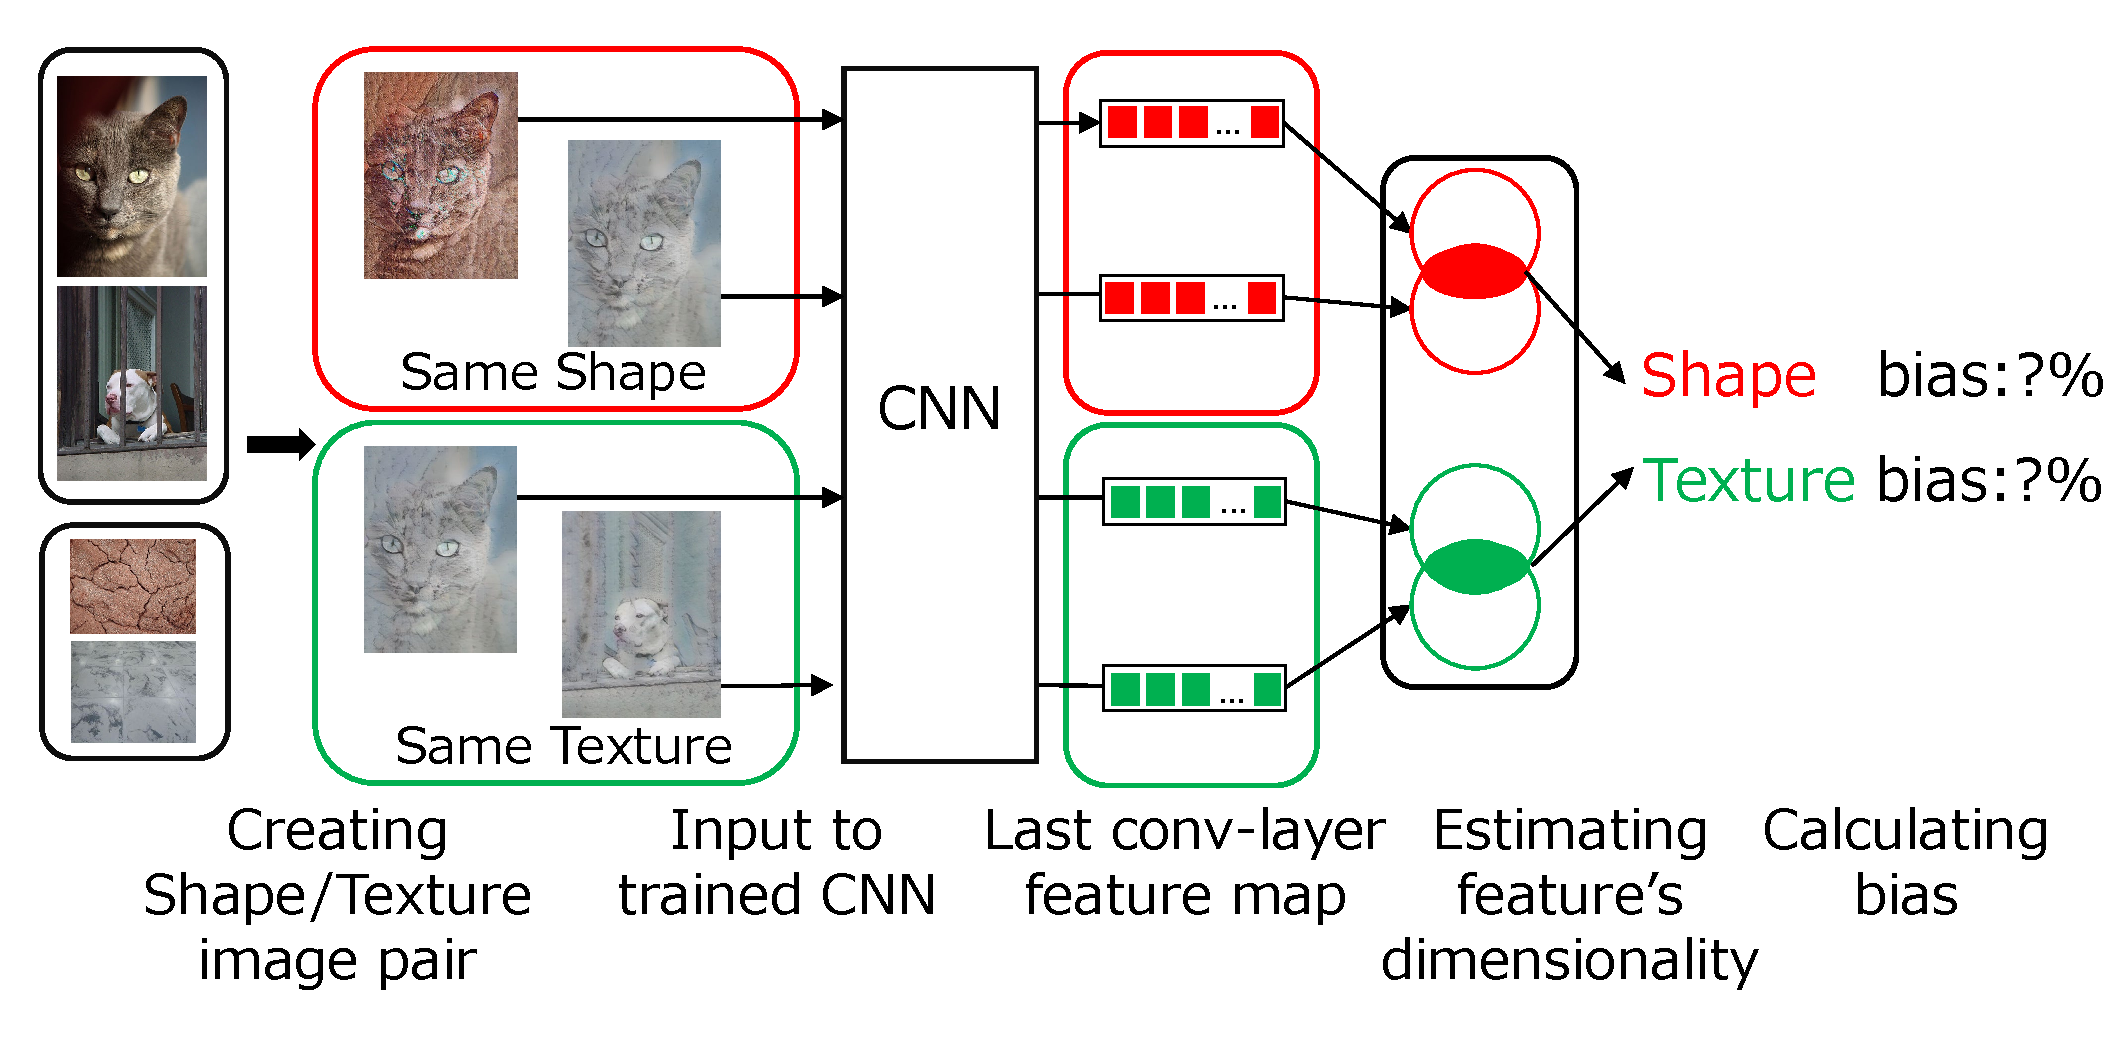
\includegraphics[width=1\columnwidth]{fig/fig2.pdf}
\caption{
%図3.Islamの方法の概要.この図は,[14]の方法で形状とテクスチャの重み付けを計算するプロセスの概要を示しています.
% CNNの学習過程における形状・テクスチャ情報の働きを解析するためのIslamの方法\cite{Islam}.
%Islamの方法の概要.この図は,[14]の方法で形状とテクスチャの重み付けを計算するプロセスの概要を示しています.
Overview of the process of calculating the shape/texture bias using the method of \cite{Islam}.
}
\label{fig:fig3}
\end{figure}

形状・テクスチャ偏重度の定量化に使用するデータセットの作成方法について述べる.この目的のために,PASCAL VOC 2012データセット~\cite{pascal-voc-2012} とDescribable Textures Dataset~\cite{cimpoi14describing}を用いる.PASCAL VOC 2012データセットからは,単一のオブジェクトを含む画像のみを選択し,Describable Textures Datasetからは,ランダムに5つのテクスチャ画像を選択する.Describable Textures Datasetから選択されたテクスチャ画像をスタイルとして使用し,PASCAL VOC 2012データセットから選択されたすべての画像に対してスタイル変換を実行する.このスタイル転送には,AdaIn transferアルゴリズム~\cite{AdaIn}を利用する.このようにして作成されたデータセットをStylized PASCAL VOC 2012(SVOC)と呼ぶ.

SVOCを用いて偏重度を定量化する方法について詳しく説明する.SVOCを使うことで,共通の形状特徴を持つ画像ペアと共通のテクスチャ特徴を持つ画像ペアをサンプリングすることができる.これらのペアを定量化したいCNNモデルに入力すると,最終的な畳み込み層のニューロンから両方の共通特徴セットに対する特徴マップペアが得られる.これらの特徴マップを用いて,以下の式から各特徴の相関係数を計算し,偏重度を求める.

実際の計算過程を述べる.形状情報が共通する画像ペアを入力して$i$番目のニューロンから得られる特徴マップペアを$z^a_i, z^b_i$ とする.それら特徴マップペアから相関係数を計算,計算された相関係数を$\rho_i^{shape}$とする.同様に同様に,テクスチャ情報が共通する画像ペアを入力し,出力される特徴ベクトルのペアから$\rho_i^{texture}$を求める.
そして,ニューロンのごとの$\rho_i^{shape}$,$\rho_i^{texture}$それぞれの総和,形状とテクスチャのとベースライン値($=ニューロン数|z|$)から,ソフトマックス関数を用いて形状とテクスチャの偏重度を決定する.

この方法は,$i$番目のニューロンがある概念(例えば形状)をエンコードしている場合に,形状情報共通した画像ペアを入力すると,$z^a_i, z^b_i$の相互情報量は高くなり,相互情報量は(1)の式のように相関係数から下界が求まることから,相関係数を用いて計算される.

\begin{align}
\operatorname{MI}\left(z_i^a, z_i^b\right) \geq-\frac{1}{2} \log \left(1-\rho_i^2\right), \quad \text { where } \rho_i=\frac{\operatorname{Cov}\left(z_i^a, z_i^b\right)}{\sqrt{\operatorname{Var}\left(z_i^a\right) \operatorname{Var}\left(z_i^b\right)}}
\end{align}

Islamらの実装では,論文内における説明とは異なり,高速化のため,ニューロンごとに$\rho_i^{shape}$,$\rho_i^{texture}$を計算していないことに注意が必要である.
    
\newpage